
\medskip

\begin{minipage}[t]{0.55\linewidth}
	Deux urnes contiennent des boules numérotées indiscernables au toucher. Le schéma ci-contre représente le contenu de chacune des urnes.
	
	\smallskip
	
	On forme un nombre entier à deux chiffres en tirant au hasard une boule dans chaque urne :
	\begin{itemize}
		\item le chiffre des dizaines est le numéro de la boule issue de l'urne D ;
		\item le chiffre des unités est le numéro de la boule issue de l'urne U.
	\end{itemize}
\end{minipage} \hfill
\begin{minipage}[t]{0.4\linewidth}
	\hfill~
	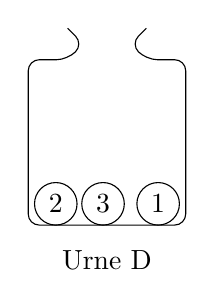
\begin{tikzpicture}[baseline = {(current bounding box.north)},x = 1cm,y=1cm]
	\draw[rounded corners] (0.5,2.5) -- (0.7,2.3) -- (0.5,2.1) -- (0,2.1) -- (0,0) --(2,0) node [pos = 0.5,below = 2mm] {Urne D}-- (2,2.1) -- (1.5,2.1) -- (1.3,2.3) -- (1.5,2.5) ;
	\draw (0.35,0.27) circle (0.27) node {2};
	\draw (0.95,0.27) circle (0.27) node {3};
	\draw (1.65,0.27) circle (0.27) node {1};
	\end{tikzpicture}
	\hfill~
	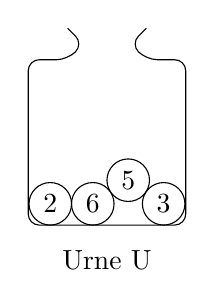
\begin{tikzpicture}[baseline = {(current bounding box.north)},x = 1cm,y=1cm]
	\draw[rounded corners] (0.5,2.5) -- (0.7,2.3) -- (0.5,2.1) -- (0,2.1) -- (0,0) --(2,0) node [pos = 0.5,below = 2mm] {Urne U}-- (2,2.1) -- (1.5,2.1) -- (1.3,2.3) -- (1.5,2.5) ;
	\draw (0.28,0.27) circle (0.27) node {2};
	\draw (0.82,0.27) circle (0.27) node {6};
	\draw (1.72,0.27) circle (0.27) node {3};
	\draw (1.27,0.57) circle (0.27) node {5};
	\end{tikzpicture}
	\hfill~
\end{minipage}

\smallskip

Exemple : en tirant la boule ~~\tikz[baseline = {(0,-3pt)}]{\draw (0,0) circle (0.3) node {1}}~~ de l'urne D et ensuite la boule ~~\tikz[baseline = {(0,-3pt)}]{\draw (0,0) circle (0.3) node {5}}~~ de l'urne U, on forme le nombre 15.
	
	\smallskip
	
	\begin{enumerate}
		\item A-t-on plus de chance de former un nombre pair que de former un nombre impair ?
		\item \begin{enumerate}
			\item Sans justifier, indiquer les nombres premiers qu'on peut former lors de cette expérience.
			\item Montrer que la probabilité de former un nombre premier est égale à $ \dfrac{1}{6} $.
		\end{enumerate}
		\item Définir un évènement dont la probabilité de réalisation est égale à $ \dfrac{1}{3} $.
	\end{enumerate}

\vspace{5 mm}

